This chapter will describe three control rod decusping methods developed as part of this work.  The first method is polynomial decusping, a simple correction based on pregenerated data.  The second method is subplane collision probabilities.  This method extends the subplane scheme by introducing a 1D collision probabilities calculation to capture subgrid information around partially inserted rods.  The final method presented here is the subray method of characteristics.  This modified form of MOC directly accounts for the partially inserted rod in the 2D MOC calculations instead of applying corrections to cross sections afterwards.

\section{Polynomial Decusping}

The polynomial decusping technique was developed to provide a fast, simple correction to the cusping problem in the MPACT code.  This technique assumes that the reactivity and power around the partially inserted rod have a predictable shape as functions of the rod position within the MOC plane.  Based on this assumption, correction factors were developed to reduce the volume fraction of control rod material and reduce the magnitude of the cusping effects.

\subsection{Correction Data Generation}

To generate this data, two different sets of calculations were required.  Both sets were done using a 3$\times$3 assembly case with a control rod in the center assembly.  The first set of calculations began with the control rod aligned with MOC plane boundaries.  The rod was then withdrawn upward through the MOC plane and simulated at different positions.  A total of 9 simulations were conducted: one with the rod aligned with the bottom of the plane, one with the rod aligned with the top of the plane, and 7 with the rod partially inserted to various depths in the plane.  The first and last calculations had no cusping effects because the rod was aligned with plane boundaries, but the remaining cases exhibited severe cusping effects.

The second set of calculations used the same problem and rod positions as the first set.  However, for the 7 partially inserted calculations, an extra MOC plane boundary was added that aligned with the control rod tip.  This eliminated rod cusping effects for the second set of calculations.  These two sets can then be compared to determine the magnitude of the cusping effects for each rod position by plotting \keff{} against rod position.

\begin{figure}[h]
    \centering
    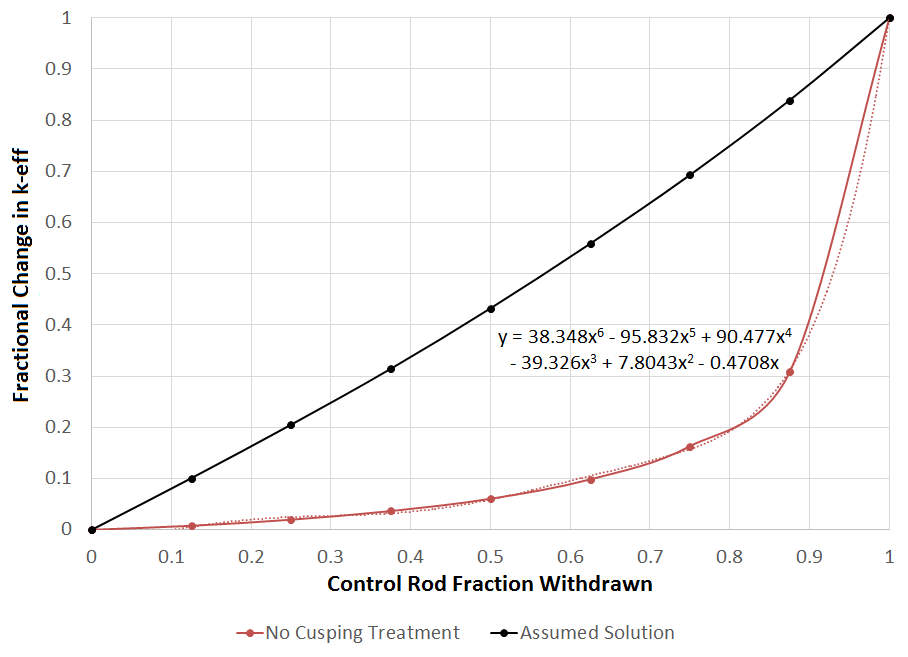
\includegraphics[width=\textwidth]{polynomial_curves.png}
    \caption{Polynomial decusping example data generation}\label{f:polynomial}
\end{figure}

Since these data need to be used to correct rod cusping for different MOC planes and reactors, the data is best plotted as a percent change in \keff{} versus a percent rod withdrawal.  An example of this is shown in Figure \ref{f:polynomial}.  The data from these calculations was then used to generate a sixth-order polynomial that approximates the shape of the rod cusping effects.  Generating this polynomial in terms of percents allows the polynomial to approximate the response for any MOC plane in any reactor.  However, the response varies significantly for different rod materials, so this process should be repeated for each unique type of control rod.  For the work presented here, polynomials were generated for three different materials: silver-indium-cadmium alloy (AIC), \bfc{}, and tungsten.  The polynomials developed for each material are shown below:
\begin{align}\label{e:polynomials}
P_{AIC}\left(V_u\right) &= 38.348 V_u^6 - 95.832 V_u^5 + 90.477 V_u^4 - 39.326 V_u^3 + 7.8043 V_u^2 - 0.4708 V_u \ ,\\
P_{B4C}\left(V_u\right) &= 46.843 V_u^6 - 117.14 V_u^5  + 109.78 V_u^4 - 47.104 V_u^3 + 9.1734 V_u^2 - 0.5527 V_u \ ,\\
P_{TUN}\left(V_u\right) &= 4.7734 V_u^6 - 14.751 V_u^5 + 19.512 V_u^4 - 12.762 V_u^3 + 4.0769 V_u^2 - 0.1505 V_u \ ,
\end{align}
where $V_u$ is the unrodded volume fraction and $P_x\left(V_u\right)$ is the corresponding percent change in \keff{} for a given rod type, with $x$ being $AIC$, $B4C$, or $TUN$.

\subsection{Correction Application}

Following the procedure in the previous section gives polynomials to approximate the shape of the cusping effects for different rod materials.  To apply these polynomials to 2D/1D calculations, the volume fractions used in the homogenization prior to 2D/1D calculations can be modified.  This homogenization is done using a simple volume weighting in the partially rodded regions:
\begin{equation}
\Sigma_x = V_u \Sigma_x^U + V_r \Sigma_x^r\ ,
\end{equation}
where $\Sigma_x$ is the cross section being homogenized, $V$ is the volume fraction, $u$ and $r$ subscripts and superscripts denote rodded and unrodded quatities, respectively, and $V_u + V_r = 1$.  It is evident from Equation \ref{e:polynomials} that cusping always lowers the value of \keff{}, so if $V_u$ is increased and $V_r$ is decreased, the rod cusping errors should be reduced.

At the beginning of the calculation, the volume fraction of the control rod is determined.  For example, if an AIC rod is 50\% inserted into a plane, the data from Figure \ref{f:polynomial} can be used to determine the expected percent change in \keff{}.  In MPACT, the approximation is made that the reference solution in Figure \ref{f:polynomial} is a straight line, resulting in a 50\% change in \keff{} from a 50\% inserted rod.  Next, the point along the polynomial which corresponds to 50\% change in \keff{} is identified.  Finally, the volume fraction which produces that value of the polynomial is used in the homogenization.  For this example, values of $V_u=0.5$ and $V_r=0.5$ would be used for a 50-50 mixture of moderator and AIC control rod without any decusping method.  To improve this solution, the model actually used would use values of approximately $V_u=0.93$ and $V_r=0.07$ to minimize the error in \keff{}.

To find the volume fraction required for improved homogenization, a root-finding method must be applied.  For the example in the previous paragraph, MPACT does this by setting $P_{AIC}\left(V_u\right) = 0.5$ in Equation \ref{e:polynomials} and moving it to the right-hand side of the equation.  Because these polynomials are smooth, monotonically increasing on the interval [0,1], and have analytic derivatives that can be easily programmed in MPACT, Newton's method \cite{2006friendlyIntroductionToNumericalAnalysis} can be easily applied to obtain the root, though other methods could be used as well.  The search is performed until the value is within 0.001 of the actual root; usually this requires only 4-5 iterations, meaning that these calculations are trivially fast compared to 2D/1D.

\section{Subplane Collision Probabilities}

The subplane scheme as it was originally conceived was used primarily to address stability issues caused by thin MOC planes in early 2D/1D codes.  While other improvements to the 2D/1D method have largely eliminated these problems, the idea of capturing subplane information using the subplane scheme can be useful for addressing partially inserted rods without substantially increasing the computational cost.  To do this, three changes were made to the basic subplane scheme: an axial correction performed during CMFD homogenization, an optional radial correction to generate improved flux profiles, and an MOC cross section correction.  A flow chart of this process is shown in Figure \ref{f:SubplaneCP-flowchart}

\begin{figure}[h]
    \centering
    \begin{tikzpicture}[node distance=2cm]

% Begin
\node (start) [startstop] {MOC Calculation};

% Pre-solve
\node (radial) [decision, right of=start, xshift=2cm] {Using 1D CP?};
\node (shape) [process, right of=radial, yshift=2.5cm, xshift=2cm] {Determine axial shape functions from previous iteration};
\node (cpm) [process, right of=radial, yshift=-2.5cm, xshift=2cm] {Perform 1D CP calculations};
\node (homogenize) [process, right of=shape, xshift=2cm,yshift=-2.5cm] {Homogenize with axially heterogeneous cross sections and flux profiles};
\node (dhats) [process, below of=homogenize,yshift=-0.5cm] {Calculate $\hat{D}$};

% Solve
\node (solve) [process, below of=dhats] {Perform CMFD eigenvalue calculation};

% Post-solve
\node (projection) [process, left of=solve, xshift=-2.5cm] {Project subplane flux to fine mesh};
\node (xs) [process, left of=projection,xshift=-2.5cm] {Rehomogenize fine mesh cross sections};

% Finish
\node (stop) [startstop, below of=xs] {Continue to 1D P$_3$ and 2D MOC};

% Basic Arrows
\draw [arrow] (start) -- (radial);
\draw [arrow] (homogenize) -- (dhats);
\draw [arrow] (dhats) -- (solve);
\draw [arrow] (solve) -- (projection);
\draw [arrow] (projection) -- (xs);
\draw [arrow] (xs) -- (stop);

% Fancy Arrows
\draw [arrow] (radial) |- node[anchor=east] {no} (shape);
\draw [arrow] (radial) |- node[anchor=east] {yes} (cpm);
\draw [arrow] (shape) |- (homogenize);
\draw [arrow] (cpm) |- (homogenize);

\end{tikzpicture}
    \caption{Calculation flow for 2D/1D with subplane collision probabilities}\label{f:SubplaneCP-flowchart}
\end{figure}

\subsection{Axial Correction}

Traditionally, the subplane scheme uses axially constant cross sections for all subplanes in each MOC plane.  When a control rod is partially inserted in the plane, a flux-volume homogenized cross section is calculated and used for each subplane.  This is done by applying Equations \ref{e:CMFDhomogTerms} usnig the axially homogenized cross sections from the MOC calculations.  This allows the subplane scheme to be used, but does little to account for the partially inserted rod.

To resolve this issue, the subplanes with the control rod use the rod cross section, and the subplane without the rod use the moderator cross section.  These cross sections are still homogenized using flux-volume weighting with fluxes from the homogenized MOC plane, but without homogenizing the cross sections axially.  Thus, Equations \ref{e:CMFDhomogTerms} are used as before, but with the unhomogenized control rod or moderator cross sections instead of the homogenized MOC cross sections.  Doing this allows both the CMFD and P$_3$ calculations to capture some of axial effects of the partially inserted rod, reducing the magnitude of the cusping errors around the rod.

\subsection{Radial Correction}

Using axially heterogeneous cross sections within an MOC plane corrects some of the cusping effects, but it does not accurately capture the radial effects of the partially inserted rod.  In reality, the radial flux shape in the rodded subplanes is completely different from the shape in the unrodded subplanes.  The MOC calculations are done on the thicker MOC planes using axially homogenized cross sections in the partially rodded regions.  This produces a radial flux shape that is not representative of either the rodded or unrodded region.  Thus, using this radial flux shape to calculate the pin-homogenized cross sections for CMFD P$_3$ introduces some error in the cross sections.

To correct the radial effects, 1D collision probabilities calculations can be used as illustrated in Figure \ref{f:SCPdecusping}.  As described in Section \ref{ss:cpm}, the CP method is used to generate flux profiles for pin cell calculations.  The MOC calculations are done using axially homogenized cross sections which produce incorrect radial flux profiles.  Thus, after the MOC calculations and before the CMFD homogenization step, standalone CP calculations can be set up to generate new radial flux profiles.  For a partially inserted rod, two calculations will be set up: one for the rodded portion and one for the unrodded portion.  Each calculation will use heterogeneous cross sections to generate a radial flux profile for the rodded or unrodded axial region.  These flux profiles are then used in place of the MOC flux when performing the homogenization described in the previous section.

\begin{figure}
    \centering
    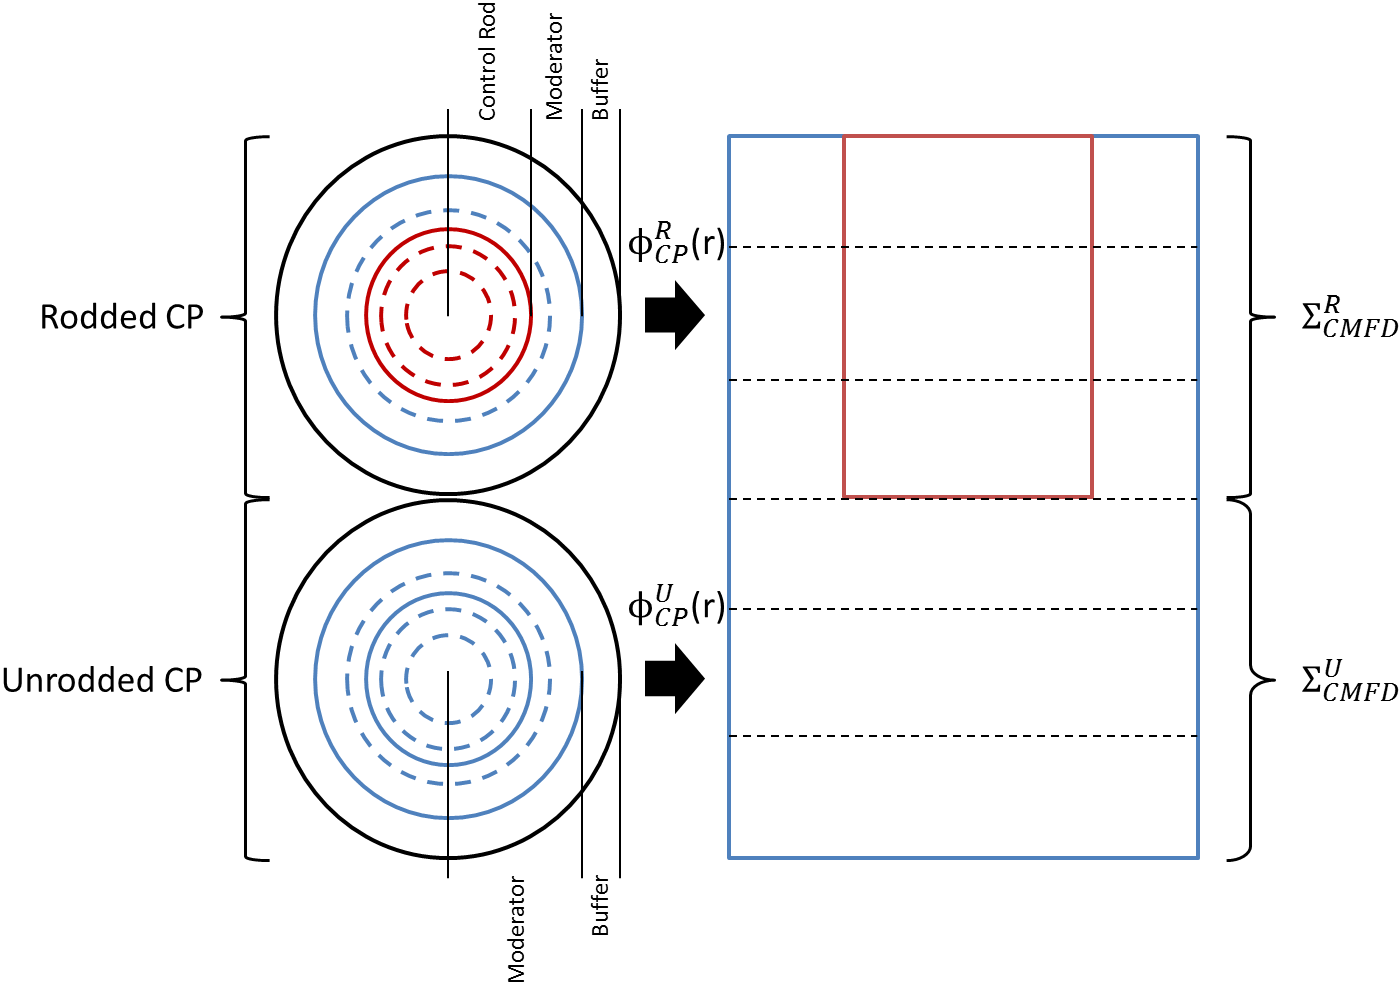
\includegraphics[width=0.8\textwidth]{CPdecusp.png}
    \caption[Subplane Collision Probabilities Illustration]{Illustration of subplane collision probabilities used on a partially inserted rod}\label{f:SCPdecusping}
\end{figure}

To set up the problem, the pin cell is cylindricized to preserve area.  The control rod and guide tube rings remain the same, but the outermost moderator region must be transformed from a rectangle to a ring.  This is done using the following equation:
\begin{equation}\label{e:cylindricize}
R_N = \sqrt{R_{N-1}^2 + \frac{L^2}{\pi}}\ ,
\end{equation}
where $R_N$ is the radius of the cylindricized rectangular moderator region, $R_{N-1}$ is the radius of the outermost ring prior to cylindricizing, and $L$ is the length of one side of the pin cell (assuming a square pin cell).  Each ring then uses the heterogeneous cross sections corresponding to the axial level being set up.  For the partially rodded regions, either rodded or unrodded cross sections will be used; for the remaining regions, the cross section will be the same for each axial level.  Finally, in order to drive the CP problem to a physical solution, a buffer region must be set up.  This is done by taking the 8 neighboring pin cells and homogenizing their sources and cross sections into an additional ring outside the final moderator ring.  This done by applying Equation \ref{e:CMFDhomogTerms} to all 8 neighboring pin cells to generate homogenized cross sections for a single region.  A variation of Equation \ref{e:cylindricize} is then applied to the buffer region:
\begin{equation}\label{e:cylindricizeBuffer}
R_{N+1} = \sqrt{\frac{8 L^2}{\pi} + R_N^2}\ ,
\end{equation}
where $R_{N+1}$ is the radius of the cylindricized buffer region and the 8 neighboring pin cells used for the buffer regions have the same dimensions $L$ as the partially rodded pin cell.

The matrix for each of these calculations is a dense $N_r \times N_r$ matrix as described in Appendix \ref{app:derivations}, where $N_r$ is around 10 or less.  It is dense because it describes the probability of neutrons born in any cell havnig a collision in every cell including itself, resulting in a completely dense matrix.  This matrix must be set up for each axial level of interest (in most cases 2), each energy group, and each partially inserted rodlet (24 per rodded assembly for the results presented in Chapter \ref{chap:results}).  Each matrix must be inverted and multiplied by a source vector.  Because the matrices are so small, these calculates are negligible compared to the cost of the full 2D/1D calculation.  Thus, the data used during homogenization can be greatly improved without incurring a significante runtime penalty.

\subsection{MOC Correction}

The final step in this decusping technique is to use the subplane information from the CMFD/P$_3$ calculations to improve the MOC calculations.  To do this, the volume-homogenized cross sections are updated each iteration using a flux-volume weighting that involves the axial flux shape from the CMFD/P$_3$ system and the radial flux shape from the CP calculations.  These are combined the same way as the nTRACER method using Equation \ref{e:nTRACERdecusping}, repeated here:
\begin{equation}
\overline{\Sigma_i} = \frac{\phi_{rad,i}^R \phi_{ax,i}^R \Sigma_i^R h^R + \phi_{rad,i}^U \phi_{ax,i}^U \Sigma_i^U h^U}{\phi_{rad,i}^R \phi_{ax,i}^R h^R + \phi_{rad,i}^U \phi_{ax,i}^U h^U}\ , \nonumber
\end{equation}
where $\Sigma_i$ is a cross section for radial ring $i$, $\phi_{rad,i}$ is the radial flux shape for ring $i$ obtained from the 1D CP calculations, $\phi_{ax,i}$ is the axial flux shape for the pin cell, and superscript $R$ and $U$ indicates a value take from either the rodded or unrodded region.  This equation can be applied to any number of subplanes for a given MOC plane, but is shown here for the simplest and most common instance of one rodded subplane and one unrodded subplane.

It is also possible to use only the axial correction and not the radial correction.  In this case, $\phi_{rad,i}^R = \phi_{rad,i}^U$ for each radial ring because the MOC flux must be used in place of the pair of 1D CP flux shapes.  This introduces some axial correction into the homogenized MOC cross sections, but no radial correction.  Chapter \ref{chap:results} will show results for ``Subplane'' (axial only) and ``Subplane + CP'' (axial and radial) to show the importance of each of these effects for different rod types.

\section{Subray Method of Characteristics}

The previous two methods are each effective in reducing the effects of rod cusping, as will be shown in Chapter \ref{chap:results}.  Despite these improvements, each method has significant drawbacks:
\begin{itemize}[leftmargin=*]
    \item \textbf{Polynomial Decusping}
    
    \begin{itemize}
        \item Corrections are limited to certain control rod materials (AIC, B$_4$C, Tungsten).
        \item Limited accuracy, especially for problems significantly different from those used to generate data.
    \end{itemize}

    \item \textbf{Subplane Collision Probabilities}
    
    \begin{itemize}
        \item CP is limited to TCP$_0$ scattering.
        \item CP implementation for non-cylindrical geometries can be complicated (e.g., BWR control blades).
        \item Instability can be introduced in the CP calculations by large transport corrections.
        \item MOC calculations are still performed using homogenized cross sections.
    \end{itemize}
\end{itemize}
The most important inaccuracy in the subplane CP method is the final point.  To fully address the partially inserted rod, it is desirable to account for the rod in the 2D MOC calculations themselves using heterogeneous cross sections.  Doing so will greatly improve the overall accuracy of the 2D/1D calculation by improving the accuracy of the transport itself.

\subsection{1D MOC Code and Problem Description}\label{ss:1dcode}

To develop this new method, a 1D MOC code was developed to investigate the behavior of angular and scalar flux near a partially inserted control rod.  This code was written in Matlab \cite{MATLAB:2016} (full source and examples scripts and inputs are included in Appendix \ref{app:1dmoc-code}) and is set up to take in a description of pins and materials to be used for the calculations.  For the geometry, a pin pitch is specified which is used for all pins.  Each pin consists of a list of radii.  Assuming a square pin cell, these pins are then transformed from cylindrical geometry to slab geometry while preserving the volume fraction of each material:
\begin{equation}\label{e:cyl2slab}
w = \frac{\pi \left(R_N^2 - R_{N-1}^2\right)}{2 L}\ .
\end{equation}
The pin pitch is the same in slab geometry as in cylindrical geometry.  Each ring is then transformed into two slabs using Equation \ref{e:cyl2slab}, where $w$ is the width of each slab.  In Equation \ref{e:cyl2slab}, $R_N$ and $R_{N-1}$ are the outer and inner radii of each ring, with $R_0=0$ for the center region in the pin cell, and $L$ is the pin pitch.  Thus, the thickness of the slabs is slightly less than the radius of each region because the volume fraction is preserved for each pin.

Each region in the problem is divided into subregions to ensure the solution is mesh-converged.  Each region is then assigned a material from a cross section library file.  This file uses the ``user library'' format supported by MPACT, which allows the user to input macroscopic cross sections for absorption, nu-fission, kappa-fission, chi, and scattering moments.  For all these calculations, the C5G7 benchmark cross sections \cite{EELewisC5G72003,EELewisC5G7extended2005} were used.  These cross sections are included in Appendix \ref{app:c5g7xs}.

For the MOC sweeps, a Gaussian quadrature \cite{HandbookOfMathFunctions1972} is used with 2, 4, 8, 16, or 32 polar angles, with half of the angles being used in each direction.  The MOC sweeps are done similarly to how they are done in MPACT, with the loop over energy groups being the innermost loop.  The code can be run as either a fixed source solver or an eigenvalue solver.  For the eigenvalue mode, power iteration is used after each MOC calculation to determine and updated \keff{}.  The fixed source mode can be used to run either a specified number of iterations or to run until the scattering source is converged below some tolerance.  This allows some flexibility on exactly what kinds of results can be obtained.

\begin{figure}
    \centering
    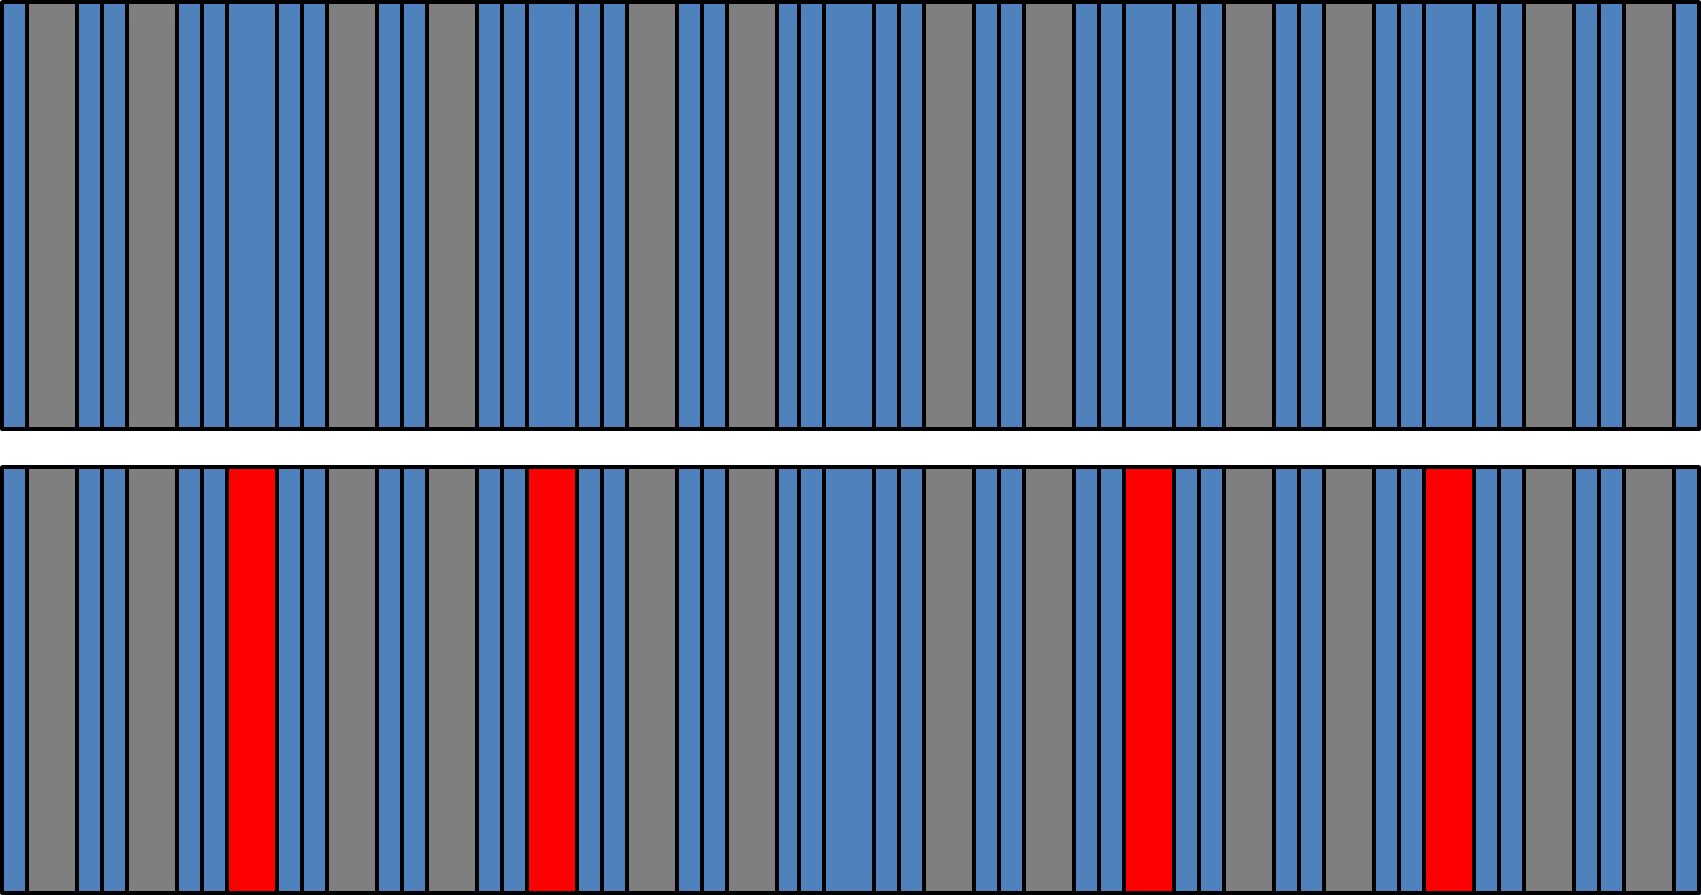
\includegraphics[width=\textwidth]{1dmoc-3x17-geom.png}
    \caption[Illustration of 1D MOC 3x17 Geometry]{Illustration of 1D MOC 3$\times$17 geometry, where the top part represents the left and right assemblies and the bottom part represents the center assembly, with materials fuel (grey), control rod/moderator mixture (red), and moderator (blue).}\label{f:1dmoc-17x17-geom}
\end{figure}

The problem used for these calculations was a 1D variation of VERA Problem 4, illustrated in Figure \ref{f:1dmoc-17x17-geom}.  The center row of pins across all three assemblies was pulled out and used for the 1D model, resulting in a row of 51 pins (17 pins across, 3 assemblies) with a pin pitch of 1.26 cm (the inter-assembly gap was neglected for this model).  The center assembly had 4 guide tubes in it which contained a mixture of moderator and control rod to represent a partially inserted control rod.  These partially rodded locations were the only part of the problem that had any material changes.  This allowed the effects of the cross section homogenization to be isolated for each calculations.

\subsection{1D MOC Investigation}

\subsubsection{Specified Total Source}

The first set of calculations performed were done using a specified total source.  To do this, the guide tubes were filled with 50\% control rod and 50\% moderator volume fraction mixture, and a full eigenvalue calculation was performed.  The total source distribution (fission and scattering) from this calculation were then passed to the the fixed source solver.  A single iteration was run using this source on three different variations of the problem: the 50-50 mixture, fully rodded, and fully unrodded.  Because the multi-group source is set up before performing any MOC sweeps, this resulted in all three of those calculations having an identical source for the MOC sweep.  The only difference between them was the cross sections used in the guide tubes.

Figure \ref{f:1dmoc-fixed-50-scalflux7} shows the scalar flux resulting from these three calculations.  The most important thing to note in this data is that the effects of the rod are very local in the MOC calculation.  Moving through the rodded pin cell, the rodded, unrodded, and mixed cases have converged back to the same shape by the time the edge of the partially rodded pin cell is reached.  Because of the exponential nature of the MOC solution in Equation \ref{e:MOCavgFlux}, if the sources are the same the two different solutions converge to each other quickly as you move away from the rod.

\begin{figure}[H]
    \centering
    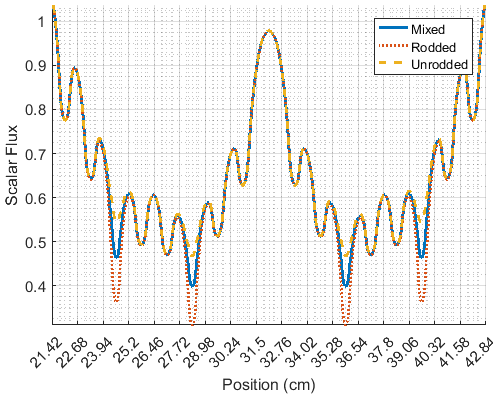
\includegraphics[width=0.7\textwidth]{1dmoc-50mix-fixedscat-scalflux7.png}
    \caption[1D MOC Group 7 Scalar Flux for Fixed Total Source]{Group 7 scalar flux comparisons for a fixed fission and scattering source calculation}\label{f:1dmoc-fixed-50-scalflux7}
\end{figure}

Figure \ref{f:1dmoc-fixed-50-angflux} shows the right-going angular flux in groups 1 (fast) and group 7 (thermal) for the center assembly using the flattest polar angle $\mu = 0.997263861849482$, where $\mu$ is the cosine of the polar angle.  This angle is shown because it has the most significant differences between the different cases; the steeper angles require fewer regions to converge to each other since the effective length of the MOC track is longer.  The group 7 angular flux behaves similarly to the group 7 scalar flux in that the effects are localized around each rod.  The three different angular flux shapes are still somewhat different at the edge of the neighboring pin cell, but these differences are nearly indiscernible upon reaching the clad and fuel in the next pin cell.  The reason for this is that the mean free path of thermal neutrons is small.  The total group 7 cross section in the moderator is about 2.65 cm$^{-1}$, which corresponds to a mean free path of about 0.38 cm, which is less than one third of the pin pitch for a typical PWR.  This combined with the exponential behavior of the MOC solution washes out the differences between the solutions quickly upon moving away from the rodded region.

\begin{figure}[H]
    \centering
    \subfigure[Group 1]{
        \centering
        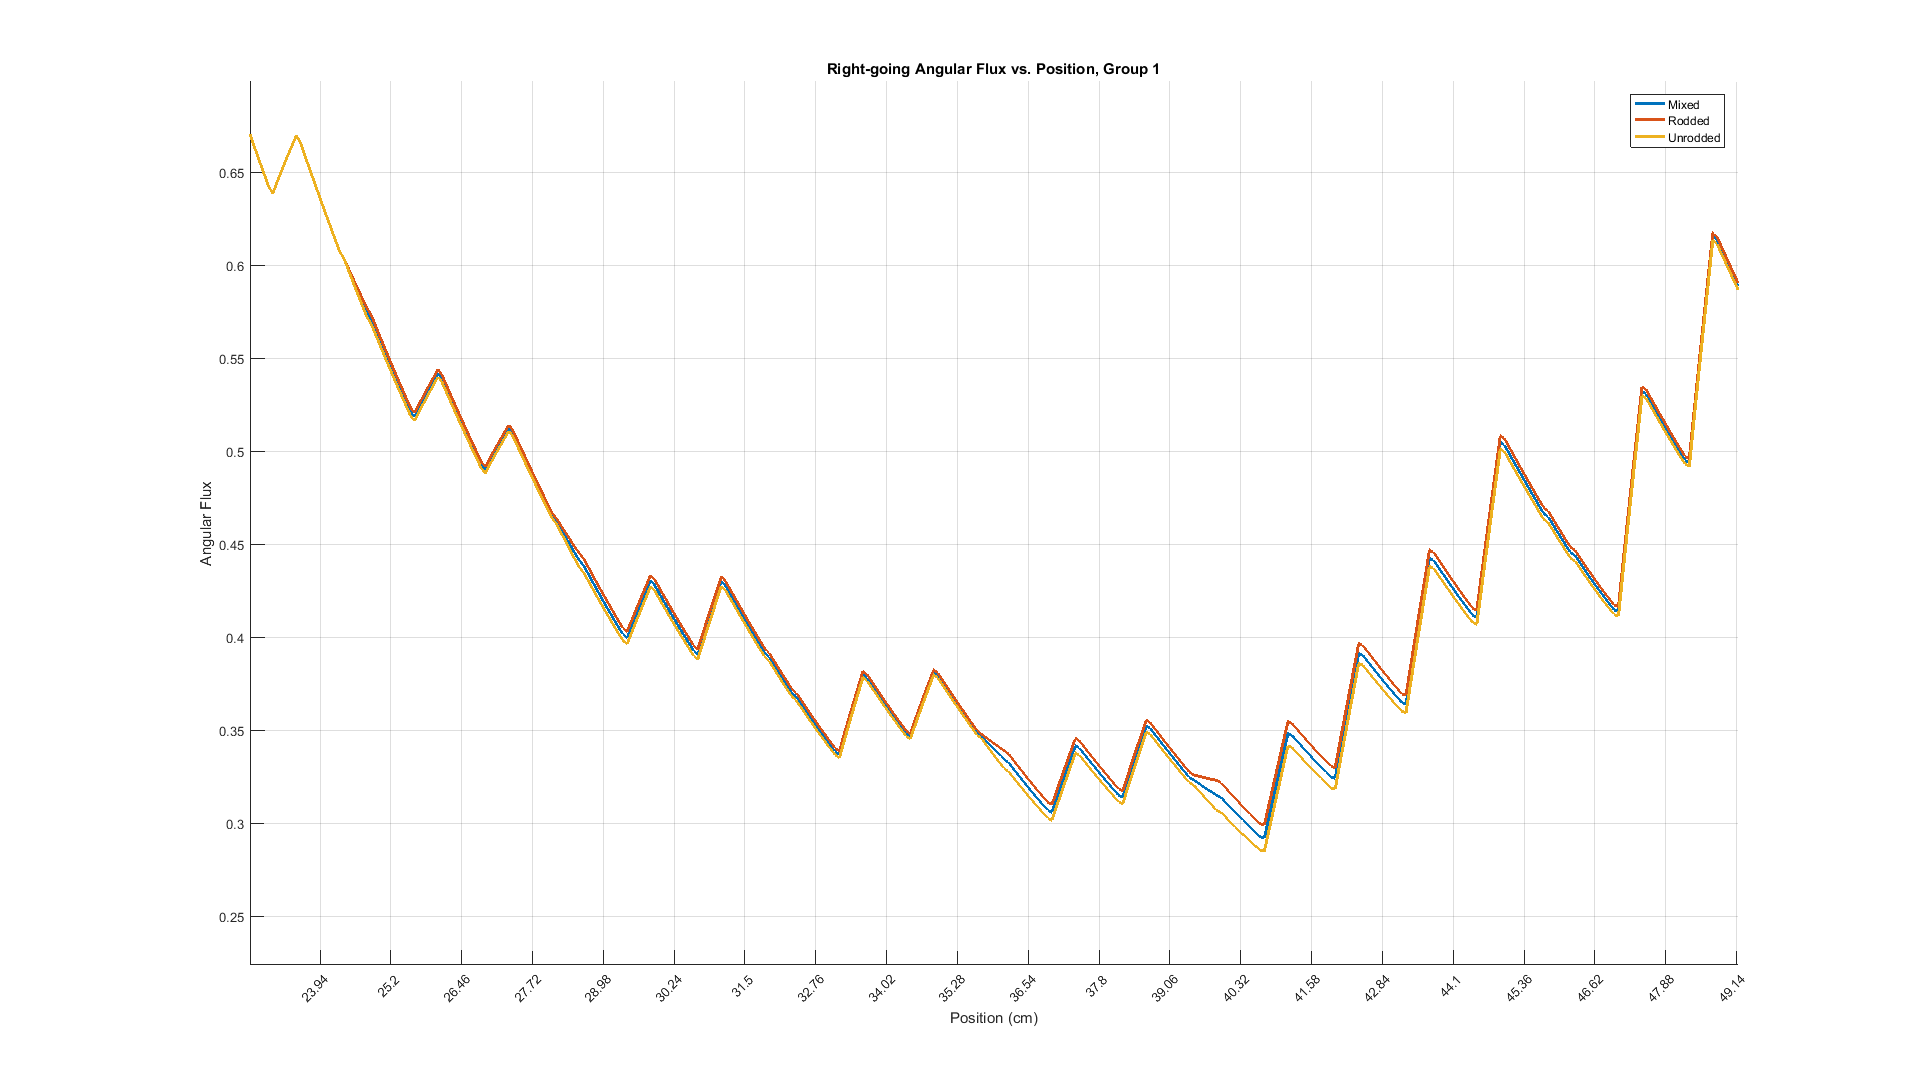
\includegraphics[width=0.48\textwidth]{1dmoc-50mix-fixedscat-angflux1.png}
        \label{f:1dmoc-fixed-50-angflux1}
    }
    \hfill
    \subfigure[Group 7]{
        \centering
        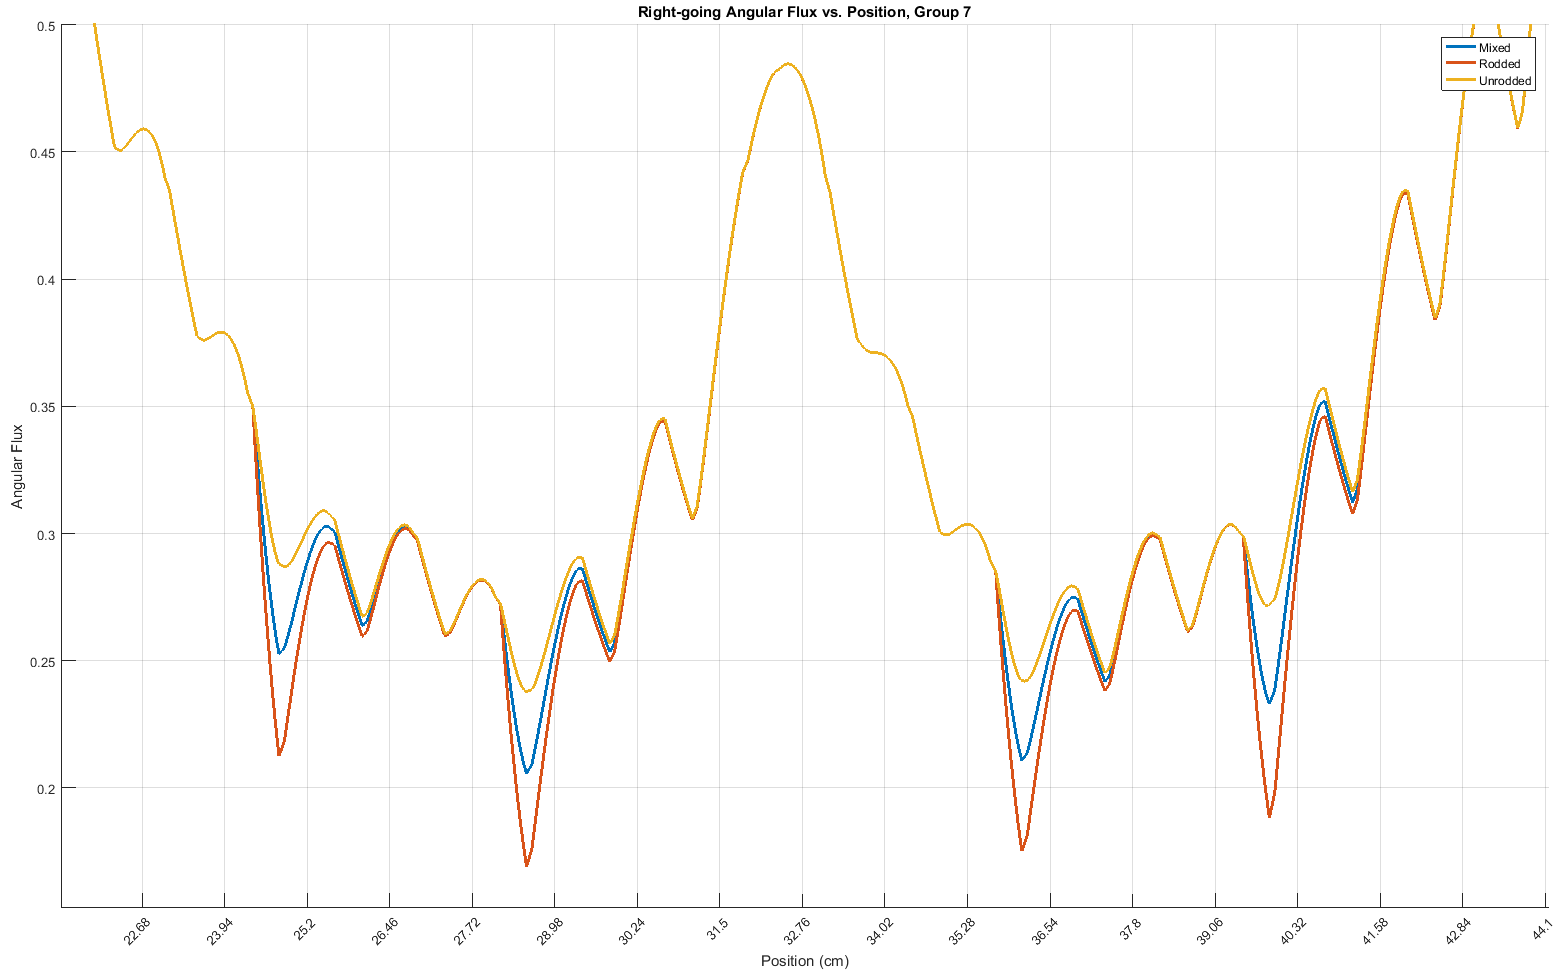
\includegraphics[width=0.48\textwidth]{1dmoc-50mix-fixedscat-angflux7.png}
        \label{f:1dmoc-fixed-50-angflux7}
    }
    \caption{Angular flux comparisons for a fixed fission and scattering source calculation}\label{f:1dmoc-fixed-50-angflux}
\end{figure}

The same cannot be said for the fast flux.  The mean free path of the fast flux is about 6.3 cm, which is the width of five pin cells.  Thus, it can be seen that each of the control rods after the first builds on the effects of the previous control rod.  Thus, the largest differences between the solutions is seen near the exit of the assembly after passing through all 4 rodded regions.  However, the differences are still small since control rods are generally thermal absorbers and have only a small impact on the flux in fast energy groups.

\subsubsection{Fixed Fission Source}

The second set of calculations that was performed used a fixed fission source, but allowed the scattering source to fully converge for each calculation.  As in the previous section, an eigenvalue calculation was completed using partially rodded cross sections.  This was done for 25\%, 50\%, and 75\% rodded cases.  For each case, a fixed fission source calculation was done with the fully rodded and fully unrodded cross sections.  This time, multiple iterations were allowed for each material to converge the scattering source.  This allows us to see the effects of the rod on the scattering source distribution without worrying about changes in the eigenvalue and fission source distribution.

\begin{figure}[h]
    \centering
    \subfigure[25\% Mixture]{
        \centering
        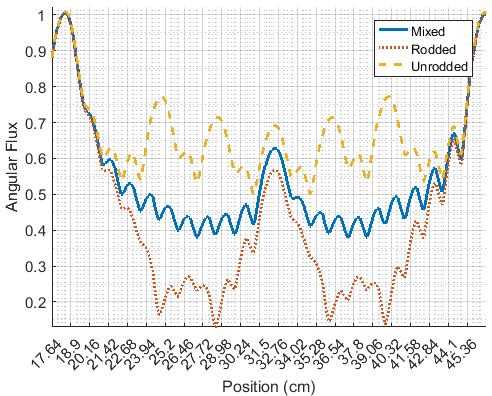
\includegraphics[width=0.48\textwidth]{1dmoc-25mix-angflux7.png}
        \label{f:1dmoc-25-angflux7}
    }
    \hfill
    \subfigure[50\% Mixture]{
        \centering
        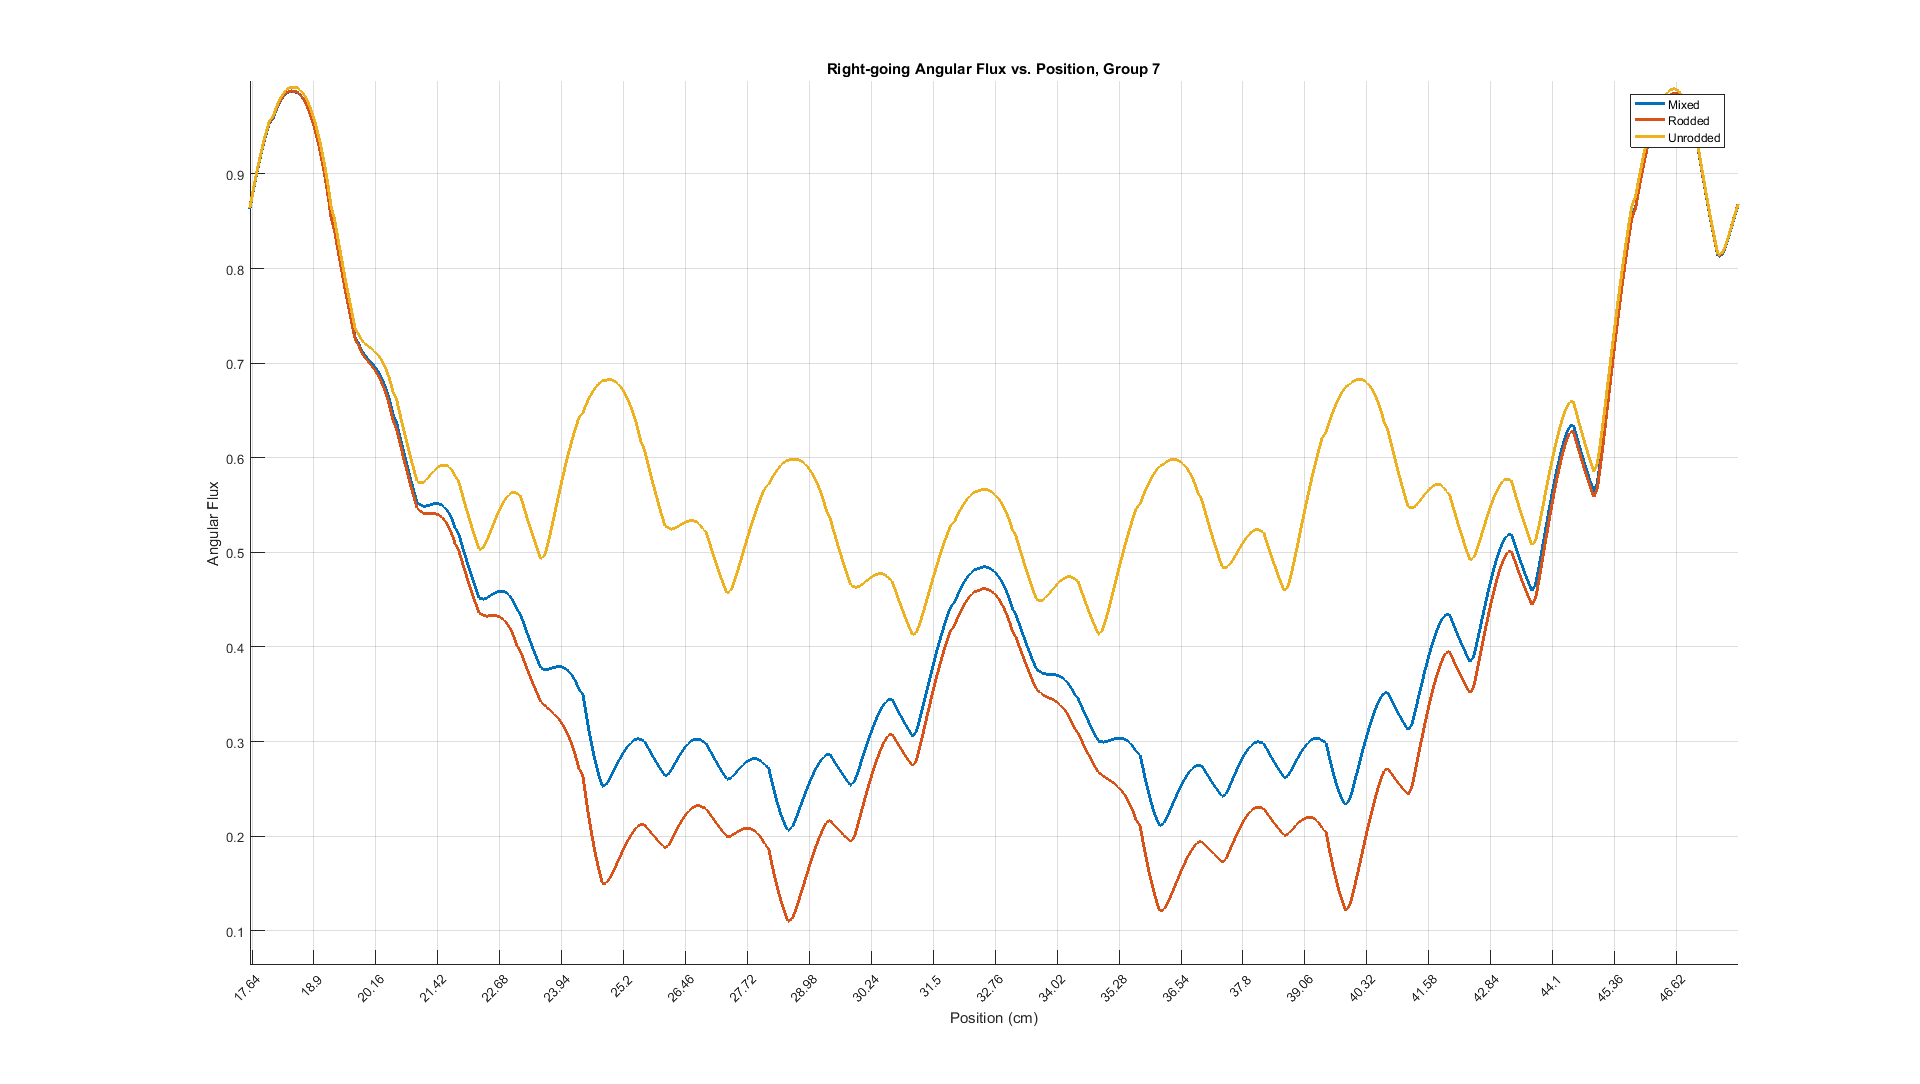
\includegraphics[width=0.48\textwidth]{1dmoc-50mix-angflux7.png}
        \label{f:1dmoc-50-angflux7}
    }
    ~
    \subfigure[75\% Mixture]{
        \centering
        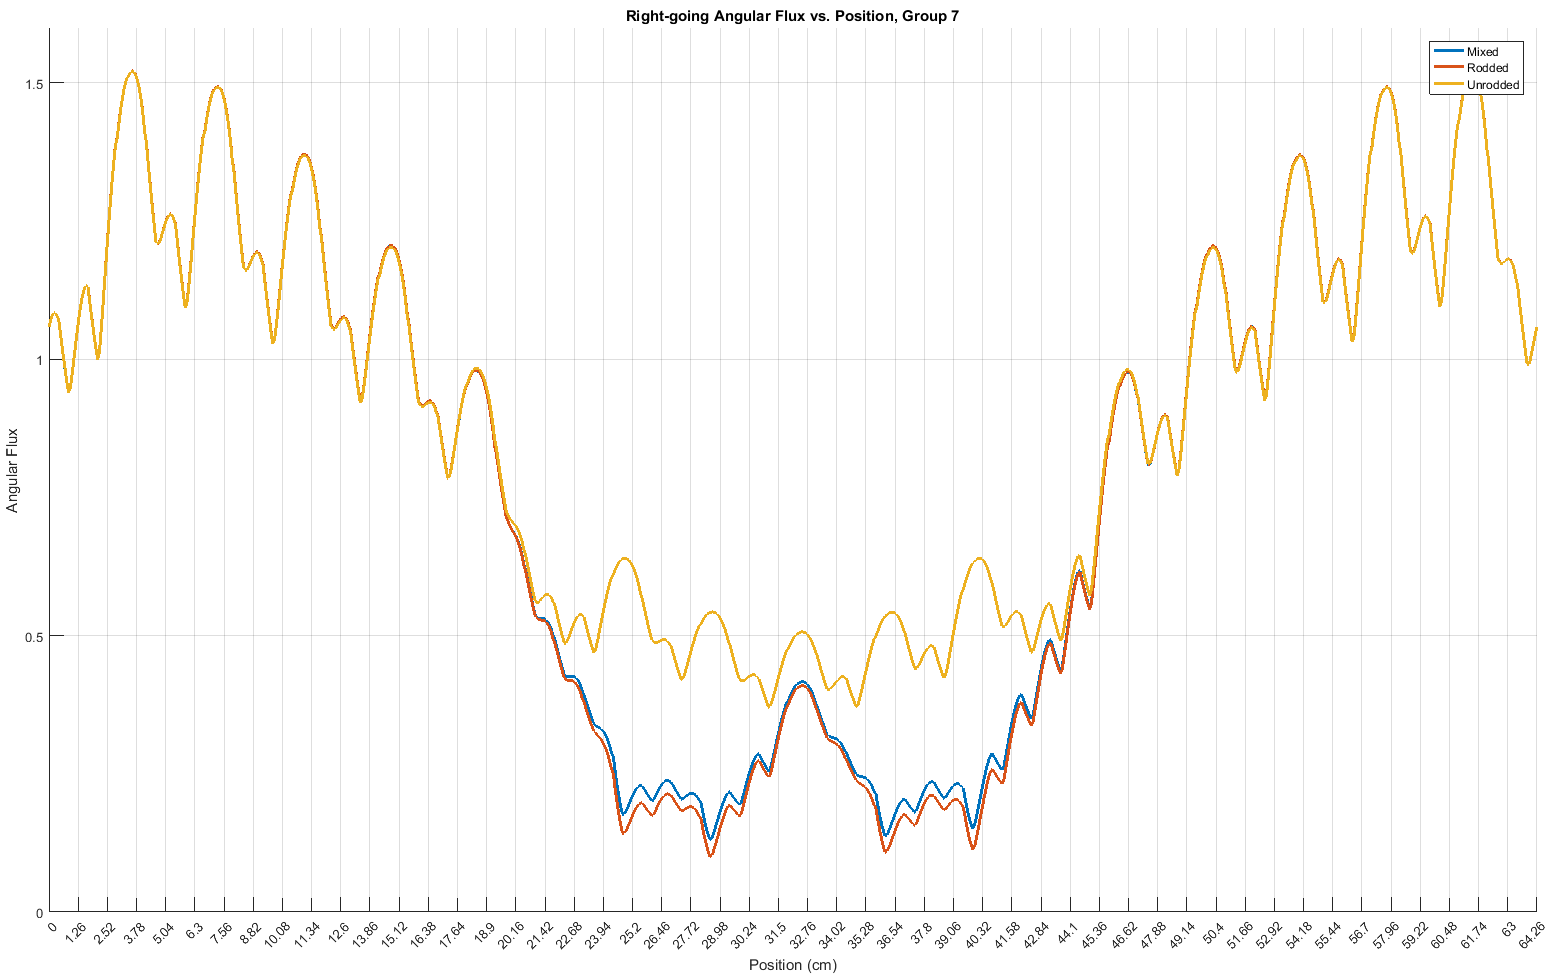
\includegraphics[width=0.48\textwidth]{1dmoc-75mix-angflux7.png}
        \label{f:1dmoc-75-angflux7}
    }
    \caption{Group 7 angular flux comparisons for 25\% and 75\% mixtures}\label{f:1dmoc-angflux7}
\end{figure}


Figure \ref{f:1dmoc-angflux7} shows the right-going group 7 angular flux comparisons for each of the three mixtures, again for the flattest value of $\mu$.  We immediately see that for each of them, the angular flux for the mixture is skewed toward the rodded result instead of being a volume-fraction--weighted average of the rodded and unrodded solutions.  For example, comparing Figures \ref{f:1dmoc-50-angflux7} and \ref{f:1dmoc-fixed-50-angflux7} shows that the angular flux is much closer to the rodded solution than when the scattering source was fixed, despite the small mean free path of thermal neutrons.  Figure \ref{f:1dmoc-angflux1} shows the same comparison for the fast flux and provides some insight into the differences in the thermal flux solutions.  The difference between the rodded, unrodded, and mixed fast fluxes are small for this calculation, similarly to the fixed total source calculations in the previous section.  However, these small differences have the effect of spreading the scattering source across the problem due to the long mean free path.  Thus, the small differences in the fast flux cause large differences in the thermal flux scattering source, which in turns effects the fission source throughout the problem.

\begin{figure}[H]
    \centering
    \subfigure[25\% Mixture]{
        \centering
        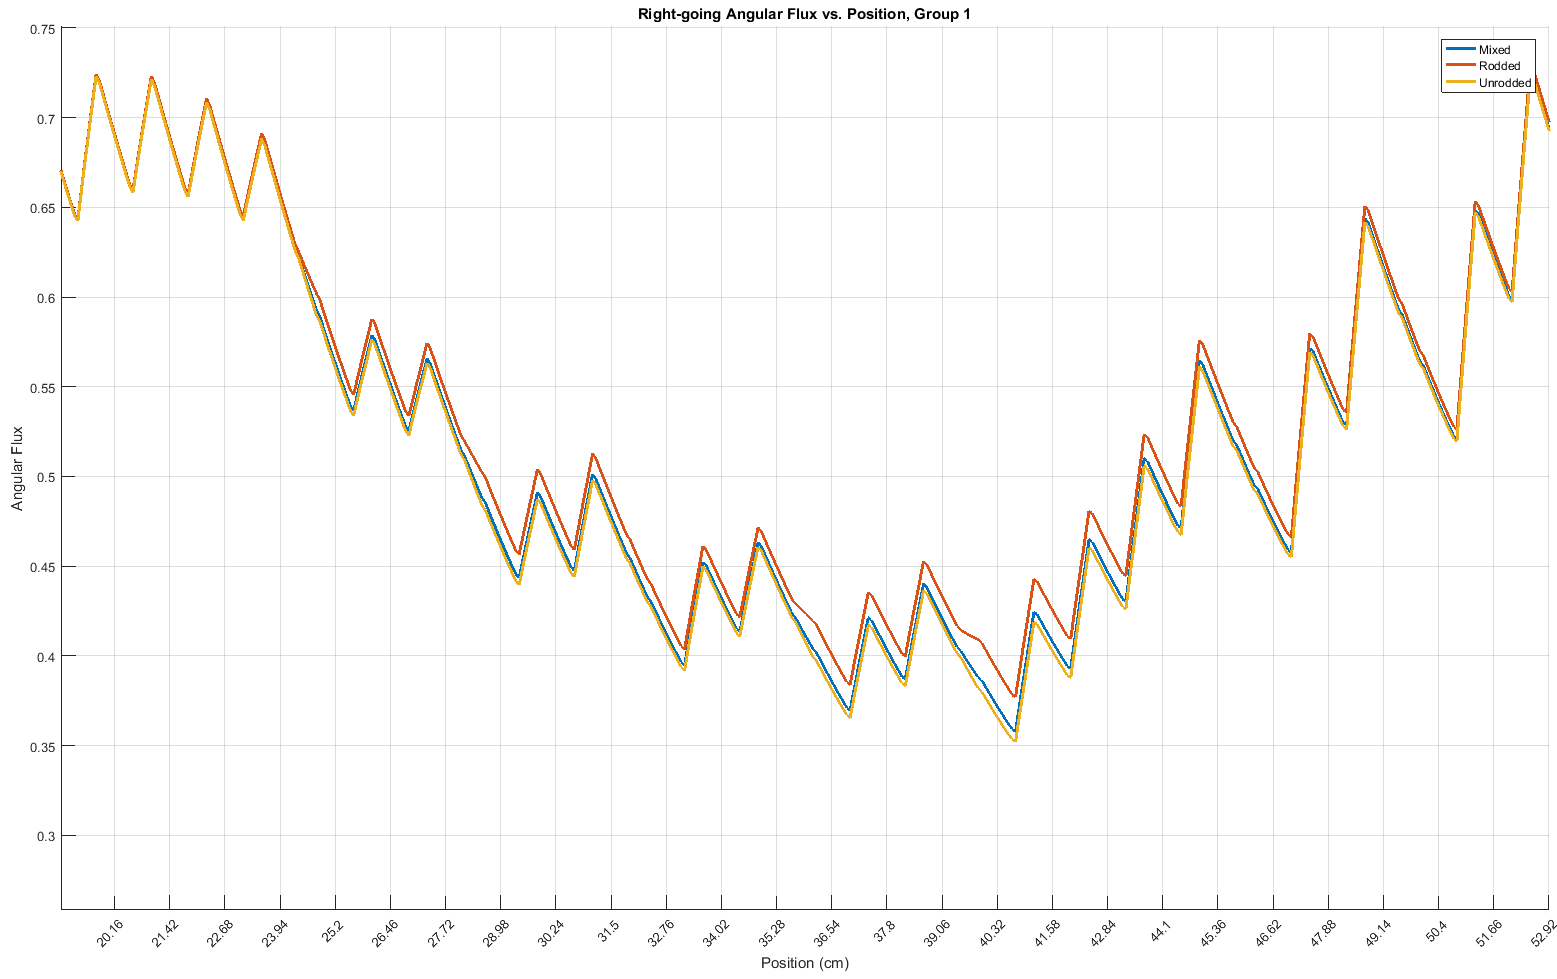
\includegraphics[width=0.48\textwidth]{1dmoc-25mix-angflux1.png}
        \label{f:1dmoc-25-angflux1}
    }
    \hfill
    \subfigure[50\% Mixture]{
        \centering
        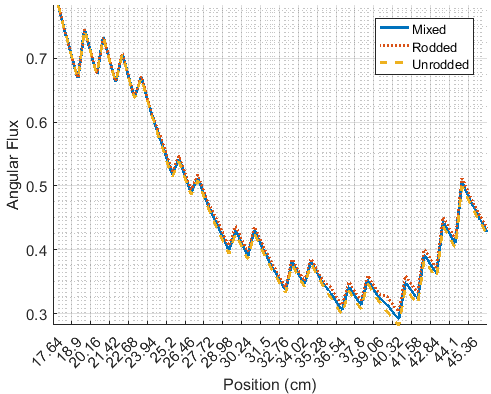
\includegraphics[width=0.48\textwidth]{1dmoc-50mix-angflux1.png}
        \label{f:1dmoc-50-angflux1}
    }
    ~
    \subfigure[75\% Mixture]{
        \centering
        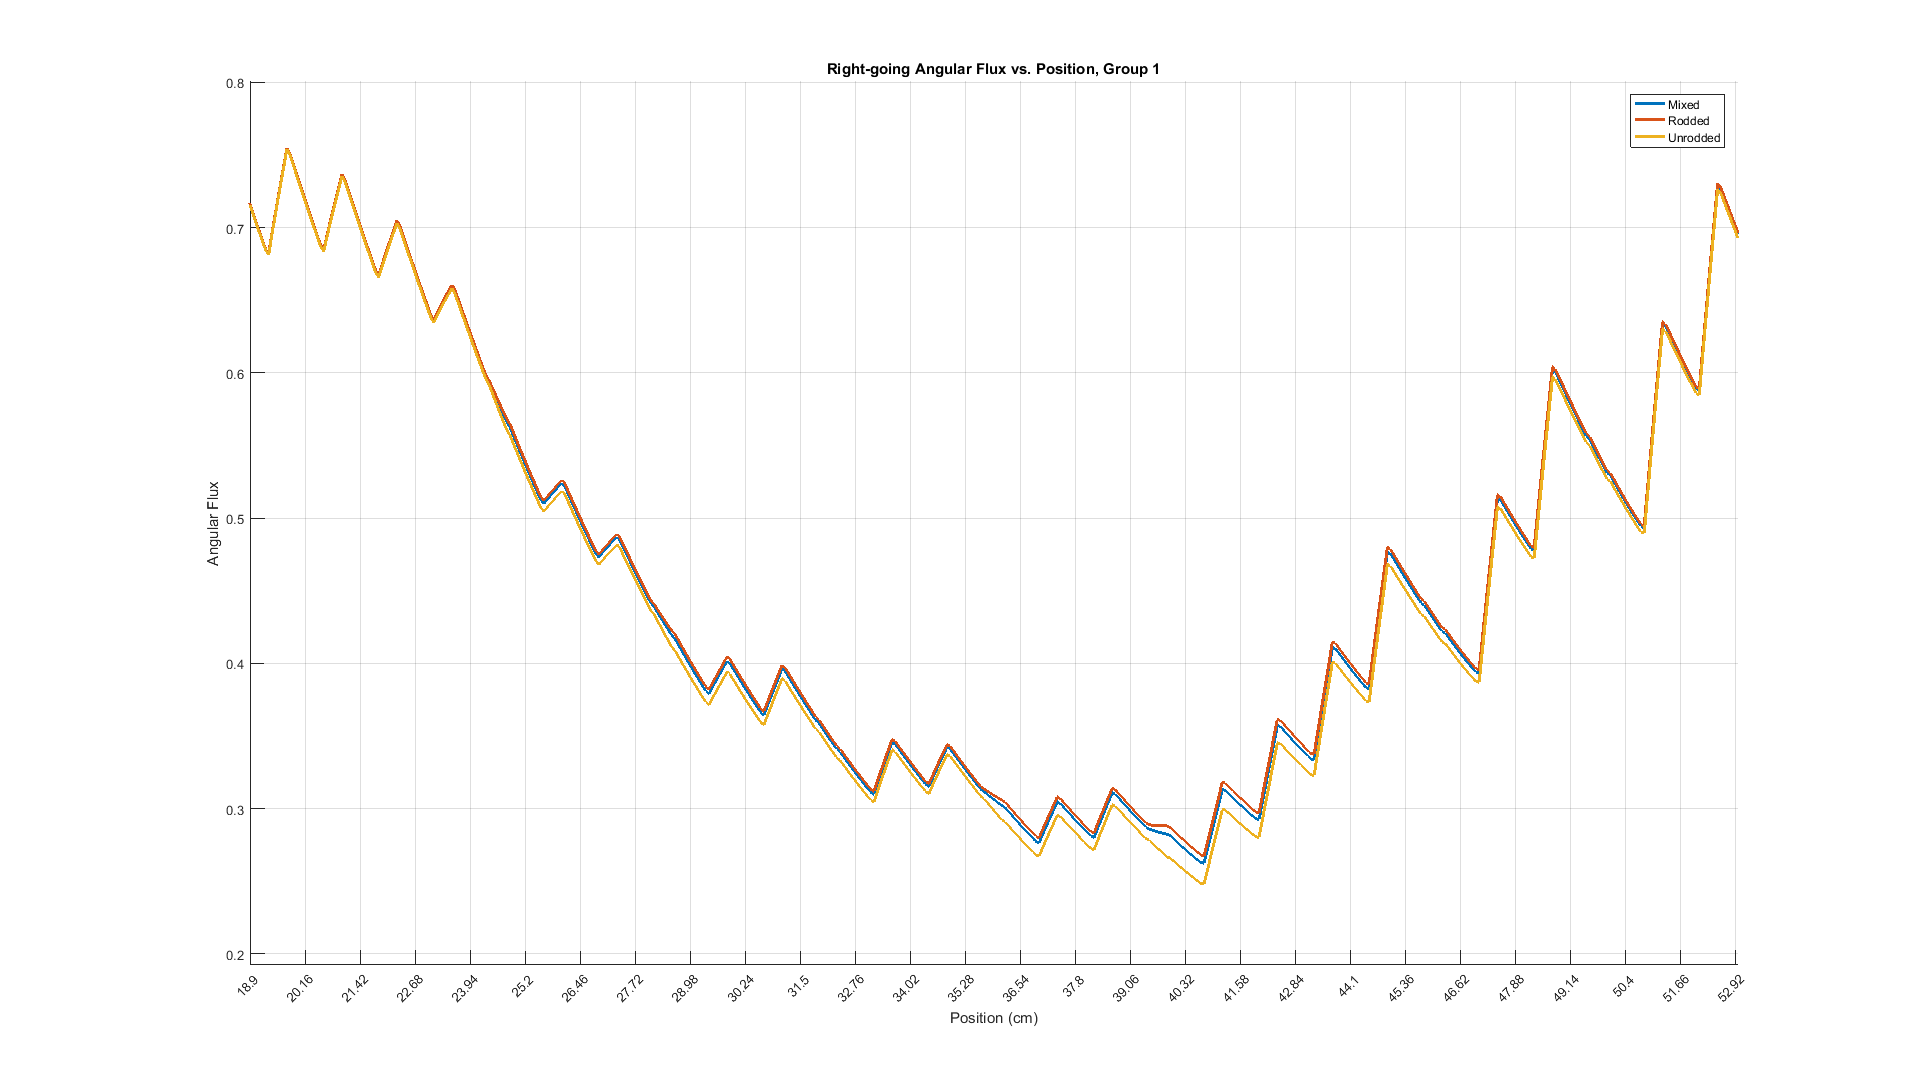
\includegraphics[width=0.48\textwidth]{1dmoc-75mix-angflux1.png}
        \label{f:1dmoc-75-angflux1}
    }
    \caption{Group 1 angular flux comparisons for 25\% and 75\% mixtures}\label{f:1dmoc-angflux1}
\end{figure}

\subsubsection{Summary}

These calculations provide several insights into what a new decusping method must be able to accomplish.  First, it must be able to account for the heterogeneous rodded and unrodded cross sections.  This is critical to obtaining an accurate shape for the thermal flux.  Second, sources must be calculated around the partially inserted rod using different scalar fluxes.  If the same scalar flux is used for both the rodded and unrodded calculations, the results are non-sensical.  Finally, the angular flux exiting the partially rodded region must accurately represent the partially inserted rod, especially for the fast flux.  If this outgoing flux is skewed incorrectly toward the rodded or unrodded fast flux solution, even small errors can have a significant impact on the scattering and fission source distributions throughout the rest of the problem.

\subsection{Subray MOC Description}

Using the results of the 1D MOC investigation described above, a new method has been developed called the subray methods of characteristics, illustrated in Figure \ref{f:subrayMOC}.  For the majority of a domain, this method will behave the same as traditional MOC.  However, when approaching a region with a partially inserted rod, the ray along which the angular flux is being solved can be split into two (or more) separate rays.  One ray will use the control rod cross section while the other will use the cross section for the material below the control rod.  The ray can be split into as many subrays as necessary to handle complicated rods or other heterogeneities, but the most common use case will split into just two subrays.  In each region where subray MOC is used, the scalar flux can be tallied using a modified form of Equation \ref{e:MOCavgFlux}:
\begin{equation}
\overline{\varphi}_{g,i,n,j} = \sum_{z=1}^Z V_z \left(\frac{q_{g,n,i,z}}{\Sigma_{t,g,i,z}} + \frac{1}{A_j\Sigma_{t,g,i,z}}\left(\varphi^{in}_{g,i,n,j,z} - \frac{q_{g,n,i,z}}{\Sigma_{t,g,i,z}}\right)\left(1 - e^{-\Sigma_{t,g,i,z} A_j}\right)\right)\ ,
\end{equation}
where $Z$ is the number of subrays used in region $i$ and $V_z$ is the volume fraction associated with subray level $z$.  Other subscripts in this equation are $g$ for energy group, $i$ for region index, $n$ for angle index, and $j$ for MOC ray index.  If the previous region also used subray, $\varphi^{in}_{g,i,n,j,z}$ is unique for each subray; otherwise, it is the same.  This equation averages the angular flux for each subray segment to obtain an axially-averaged, segment-averaged angular flux, which is then used to calculate the scalar flux.  Furthermore, the subray angular fluxes can also be used to calculate the scalar flux for these subregions to generate subregion source terms for the subsequent iteration.

After passing completely through the partially rodded regions, the subray angular fluxes can be recombined into a single ray using the volume fractions associated with each subray:
\begin{equation}
\varphi^{out}_{g,i,n,j} = \sum_{z=1}^Z V_z \left(\varphi^{in}_{g,i,n,j,z}e^{-\Sigma_{t,g,i,z} A_j} + \frac{q_{g,i,n,z}}{\Sigma_{t,g,i,z}}\left(1 - e^{-\Sigma_{t,g,i,z}A_j}\right)\right)\ ,
\end{equation}
where $\varphi^{out}_{g,i,n,j}$ is the axially averaged outgoing angular flux at the end of track $j$ for direction $n$, region $i$, and energy group $g$.  The errors introduced from this are minimal due to the exponential nature of the MOC ray calculations.  After the rod, both subrays have the same cross section again and the axial shape of the sources begins to flatten out.  Because of this, the rays then exponentially converge toward each other.  Thus, as long as an appropriate amount of distance is left between the end of the partially rodded region and the recombination point, minimal errors are introduced.  This is discussed in more detail in Section \ref{sss:recombination}.

\begin{figure}
    \centering
    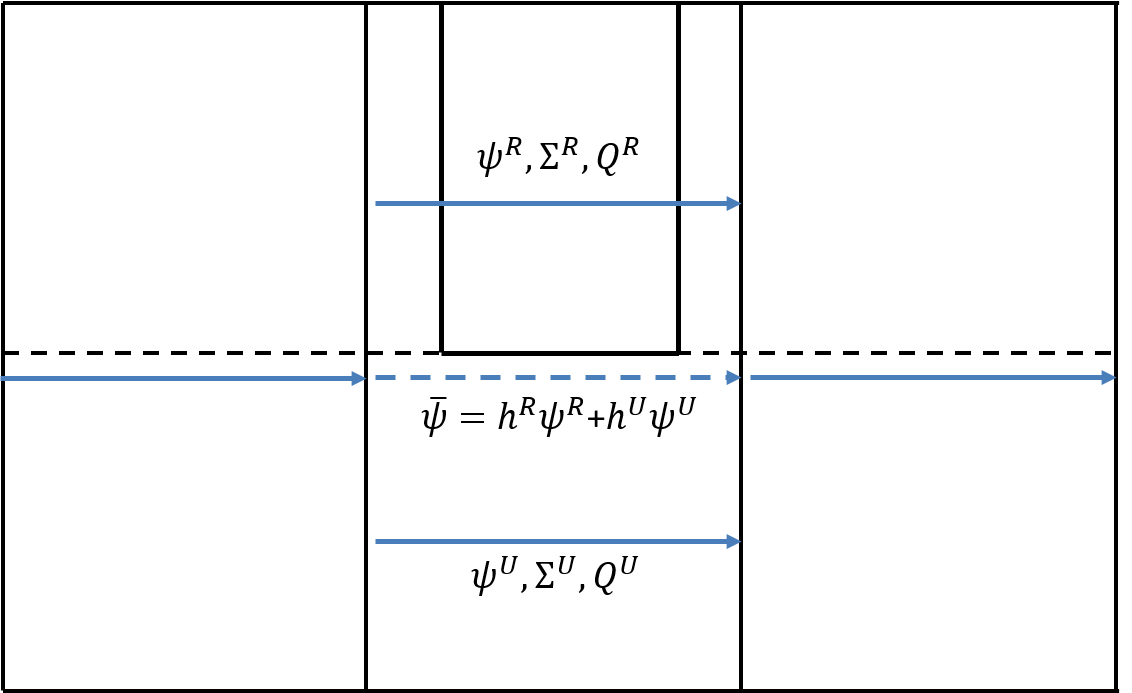
\includegraphics[width=0.8\textwidth]{sub-ray_illustration.png}
    \caption[Subray MOC Illustration]{Illustration of subray method of characteristics for partially inserted rod}\label{f:subrayMOC}
\end{figure}

This method should accurately capture the cross section and source effects around the partially inserted rod by using subrays.  Furthermore, recombining the outgoing fluxes after the rod should provide a more accurate outgoing flux than that calculated from a homogenized cross section.  This method addresses all the insights gathered from the 1D MOC investigation.  Furthermore, it addresses all the limitations of the polynomial and subplane collision probabilities decusping techniques discussed earlier in this chapter.

\subsection{MPACT Implementation}

Implementation of subray MOC in the 1D MOC code is straightforward since the code is small and uses only power iteration.  Implementing the method in the 2D/1D code MPACT is significantly more complicated.  First, even for single-plane 2D cases, MOC calculations can be expensive.  Because of this, the MOC sweep kernels need to be modified to use subray in such a way that the kernels will still be well optimized for the subray calculations.  When moving from 2D to 2D/1D other complexities are introduced from the 3D CMFD and 1D P$_3$ calculations that have to be correctly incorporated in the subray MOC calculations.  The following sections discuss some of the details of how this is done.

\subsubsection{MOC Sweeper Modifications}


Implementing a subray MOC sweeper in MPACT presents some difficulties since MPACT was not designed with these types of subgrid methods in mind.  The MOC sweepers have been optimized to ensure that the rays are swept in the most efficient way possible.  The long rays are set up once up front, then they are swept in a separate loop with no branching statements to ensure the hardware is performing the calculations as quickly as possible.  Subray MOC naturally introduces branching statements that would destroy this efficiency.

\begin{figure}[h]
    \centering
    \begin{tikzpicture}[node distance=2cm]

% Begin
\node (start) [startstop] {Calculate sources, set $n=0$};

% Solve
\node (longrays) [process, below of=start, yshift=-1cm] {Loop over long rays; $n=n+1$; $z=0$};
\node (subrays) [process, right of=longrays, xshift=2.5cm] {Loop over long rays; $z=z+1$};
\node (construct) [process, above of=subrays, yshift=0.5cm] {Construct long ray $n$, store $q$ and $\Sigma_t$ for each segment};
\node (expTable) [process, right of=construct, xshift=2.5cm] {Calculate exponential for each segment, polar angle, energy group};
\node (sweep) [process, below of=expTable, yshift=-1cm] {Loop over polar angles, segments, energy groups};
\node (track) [process, below of=sweep, yshift=-1.5cm] {For each polar, segment, and group: calculate average/outgoing angular flux, tally scalar flux and surface currents};
\node (endSubray) [decision, left of=track, xshift=-2.5cm] {$z \? N_{subrays}\left(n\right)$};
\node (endRay) [decision, left of=endSubray, xshift=-2.5cm] {$n \? N_{rays}$};
\node (postprocess) [process, below of=endRay, yshift=-2cm] {For partially rodded regions, apply Equation \ref{e:subrayPostProcess}};

% Finish
\node (stop) [startstop, right of=postprocess, xshift=2.5cm] {End planar sweep};

% Basic Arrows
\draw [arrow] (start) -- (longrays);
\draw [arrow] (longrays) -- (subrays);
\draw [arrow] (subrays) -- (construct);
\draw [arrow] (construct) -- (expTable);
\draw [arrow] (expTable) -- (sweep);
\draw [arrow] (sweep) -- (track);
\draw [arrow] (track) -- (endSubray);
\draw [arrow] (postprocess) -- (stop);

% Fancy Arrows
\draw [arrow] (endSubray) -- node[anchor=east] {no} (subrays);
\draw [arrow] (endSubray) -- node[anchor=south] {yes} (endRay);
\draw [arrow] (endRay) -- node[anchor=west] {no} (longrays);
\draw [arrow] (endRay) -- node[anchor=west] {yes} (postprocess);

\end{tikzpicture}
    \caption{Calculation flow for 2D MOC sweep of a single plane with subray}\label{f:MOC-sweep-subray-flowchart}
\end{figure}

To get around this, an extra loop was added just inside the loop over long rays.  This is illustrated in Figure \ref{f:MOC-sweep-subray-flowchart}, which is a modified form of Figure \ref{f:MOC-sweep-flowchart}.  This loop goes from one to the number of subrays for that long ray.  For most long rays, this number will just be one, meaning that long ray gets swept exactly one time.  The results of the sweep for those long rays is exactly the same as if subray MOC were not being used.  For the long rays that intersect with a partially rodded region, the ray is constructed and swept multiple times (usually just twice unless the partially inserted rod has multiple axial regions).  During the sweep, volume fractions are used to tally the surface currents for CMFD and the region-wise scalar fluxes outside the partially rodded region as shown in Equation \ref{e:subrayTallies}:
\begin{subequations}\label{e:subrayTallies}
\begin{equation}
\phi_{g,i} = \phi_{g,i} + \overline{\varphi}_{g,i,n,j,z} w_n V_z\ ,
\end{equation}
\begin{equation}
J_{g,s} = J_{g,s} + \varphi_{g,i,n,j,z}^{out} \mu_n w_n V_z\ ,
\end{equation}
\end{subequations}
where $\phi_{g,i}$ and $J_{g,s}$ are the region $i$ scalar flux and surface $s$ net current, $V_z$ is the volume fraction associated with subray $z$, $\overline{\varphi}_{g,i,n,j,z}$ and $\varphi_{g,i,n,j,z}^{out}$ are the average angular flux along track $j$ and the outgoing angular flux at the end of track $j$, and $\mu_n$ and $w_n$ are the quadrature azimuthal angle cosines and weights, respectively.  Inside the partially rodded region, the scalar fluxes are tallied into two separate regions (one rodded, one unrodded) as described in Section \ref{sss:2d1dMOCsweepAlgorithm}.  This allows these subregion scalar fluxes to construct the scattering source for the next iteration.  After the sweep of the full plane is complete, the subregion scalar fluxes are combined using volume fractions as a post-processing step:
\begin{equation}\label{e:subrayPostProcess}
\phi_{g,i} = \sum_{z=1}^Z V_z \phi_{g,i,z}\ ,
\end{equation}
where $\phi_{g,i}$ is the scalar flux for group $g$ and region $i$ for the full-height MOC plane, $V_z$ is the subregion volume fraction for axial level $z$, and $\phi_{g,i,z}$ is the subregion scalar flux for group $g$, region $i$, and axial level $z$.

This approach has the drawback of duplicating several of the long rays.  For problems discussed in Chapter \ref{chap:results}, we can reasonably expect around 20-30\% of the long rays to intersect a partially rodded region.  However, this approach allows the MOC sweeper kernels to maintain a high degree of efficiency during the calculations.  Furthermore, based on duplicating 30\% of the long rays, we could expect a 30-40\% speedup compared with simply having 2 separate MOC planes to resolve the partially inserted rod.  Thus, taking this approach allows subray MOC to be implemented and tested without rewriting MPACT while still attaining significant speedup.

\subsubsection{Subregion and Recombination Selection}\label{sss:recombination}

Before performing the subray MOC sweeps, it must be determined which long rays will be duplicated.  This is done by examining the mesh for partially rodded regions.  Due to the source effects described previously, whenever a partially rodded region is identified, all other regions in that pin cell are also flagged as partially rodded.  This allows the axial shape of the source in the surrounding moderator region to also be resolved.

\begin{figure}[h]
    \centering
    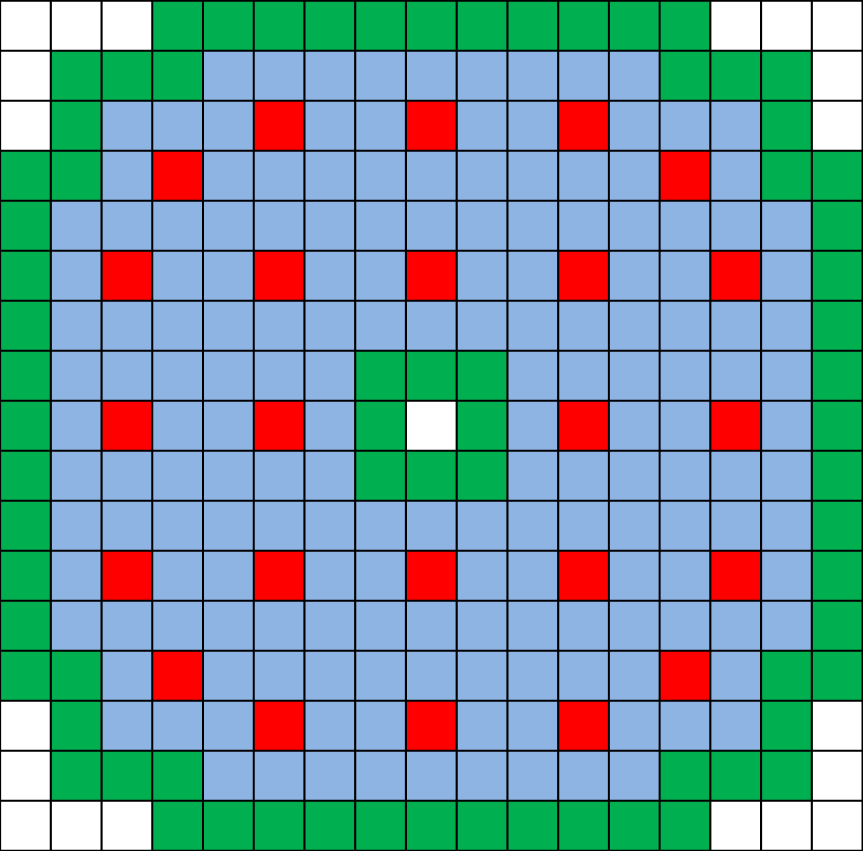
\includegraphics[width=0.8\textwidth]{recombination.png}
    \caption{Pin cells in 17$\times$17 assembly using subray MOC for recombination flags of 0 (red), 1 (blue), 2 (green), and 3 (white).}\label{f:recombination}
\end{figure}

After identifying these regions, neighboring pins can also be flagged.  As more rings of neighboring pins are added, the solution should grow closer to that of 2 separate MOC planes.  In MPACT, this was implemented via a user-defined recombination flag.  A value of 0 will only mark partially rodded regions; a value greater than 0 will add that number of rings around the partially rodded pin cell.  Once all these regions are identified, any long ray that passes through any of these regions will be swept multiple times using subray MOC.  Some of these rays will not actually intersect the control rod at all, but will serve to resolve the source effects surrounding the rods.  The rays will ``split'' upon entering any of the flagged regions and will recombine only upon entering a non-flagged region.  In Figure \ref{f:recombination}, a recombination value of 0 will use subray only for the red pins, which actually have partially inserted control rods; a value of 1 will use subray for red and blue pins; a value of 2 will use subray for red, blue, and green pins; and a value of 3 will use subray for the entire assembly.  Regardless of the value, regions in neighboring assemblies will not be flagged unless those assemblies also have partially inserted control rods.

Because the current implementation in MPACT duplicates the whole long ray, the rays are not actually recombined until the problem boundary.  However, the logic to only store axially varying sources for certain regions causes this implementation to produce identical answers compared with a more advanced implementation which actually splits and recombines each long ray while sweeping it.  The results obtained using this implementation are therefore exactly what is expected from subray MOC, though the efficiency is worse.

\subsubsection{Subplane CMFD and \texorpdfstring{P$_3$}{P3}}

Another consideration that must be made concerns the interactions between the subplane CMFD/P$_3$ calculations and subray MOC.  In theory, one could use subray MOC in 2D/1D without using the subplane scheme.  However, the fluxes used to calculate the sources for the MOC calculations would be the same for each subregion in an MOC region, limiting the accuracy of the subray MOC calculations.  Instead, it is better to modify the projection procedure described in Section \ref{sss:cmfdProj} to provide an axial shape in the MOC regions.  For each MOC subregion, an axial scaling factor is generated using Equation \ref{e:subplaneScalingFactor}.  The full-height MOC fluxes are multiplied by this scaling factor in each subregion.  These values are then used to calculate the scattering and fission sources for the subray MOC calculations.  Following this procedure produces more accurate sources and ensures that the volume-averaged flux in each CMFD cell is preserved by both the full-height MOC regions and their subregions.

Furthermore, the axial P$_3$ calculations are also done on the subplane mesh.  The regular MOC regions will use currents at the top and bottom of the MOC plane to calculate the axial TL source.  If the subplanes are aligned with the control rod, then currents are also available at the top and bottom of each of the subregions used by subray MOC using Equation \ref{e:axialTL}.  This allows a more accurate axial shape for the axial TL source, which changes especially quickly in the vicinity of a control rod tip.  Thus, using the subplane scheme will improve the accuracy of all three sources used by MOC in the 2D/1D method: scattering, fission, and axial TL.

It should also be noted that as when using subplane CMFD, the radial $\hat{D}$ coupling coefficients should be calculated on the full-height MOC mesh using Equations \ref{e:CMFDcouplingCoeffs}.  Since much of the MOC calculations are done on this mesh, it is more stable to calculate all radial $\hat{D}$ terms on this mesh.  In theory, the radial $\hat{D}$ terms could be calculated separately for each subplane since the subregion fluxes were calculated during the subray MOC sweep, but this subgrid information is only available in the vicinity of the partially inserted rod, making it more stable to use teh full-height fluxes.  The axial $\hat{D}$ terms are calculated on the subplanes using the results of the axial P$_3$ calculations as described in Chapter \ref{chap:2d1d} with no modifications to account for subray MOC.

\section{Summary}

This chapter presented 3 new rod decusping techniques for the 2D/1D method.  These techniques vary in complexity and expected accuracy, but each of them captures some of the effects of the partially inserted control rod.  The following chapter will present the results of calculations using each of these methods and provide futher discussion on the strengths and limitations of each method.